% Компіляція: lualatex -shell-escape main.tex
\documentclass[12pt,a4paper]{article}

\usepackage{fontspec}
\usepackage{polyglossia}
\setdefaultlanguage{ukrainian}
\setmainfont{NewComputerModern10}
\setmonofont{Noto Sans Mono}[Scale=0.82]

\usepackage{amsmath,amssymb,booktabs,caption,enumitem,float,geometry,graphicx,hyperref,minted,microtype,tikz,xcolor,titlesec}
\usetikzlibrary{arrows.meta,positioning,shapes.geometric}
\geometry{left=2cm,right=2cm,top=2cm,bottom=2cm}
\setlength{\parindent}{1.25cm}
\setlength{\parskip}{0pt}
\setlength{\emergencystretch}{3em}
\linespread{1.0}
\usemintedstyle{vs}
\setminted{linenos,breaklines,frame=single,fontsize=\small,tabsize=4}
\captionsetup{font=small,labelfont=bf,labelsep=endash}
\titleformat{\section}{\normalfont\fontsize{14}{16}\selectfont\bfseries\centering}{\thesection.}{0.6em}{}
\titleformat{\subsection}{\normalfont\fontsize{12}{14}\selectfont\bfseries\centering}{\thesubsection.}{0.6em}{}
\titlespacing*{\section}{0pt}{1.4em}{0.65em}
\titlespacing*{\subsection}{0pt}{1.1em}{0.45em}

\newcommand{\studentName}{Давидчук А. М.}
\newcommand{\studentGroup}{ІО-41}
\newcommand{\recordBook}{4106}
\newcommand{\teacherName}{Баран Д. Р.}
\newcommand{\reportYear}{2026}
\newcommand{\img}[2]{\begin{figure}[H]\centering\includegraphics[width=#2\textwidth]{#1}\end{figure}}
\newcommand{\methodpair}[3]{%
\begin{figure}[H]\centering
\begin{minipage}[t]{0.48\textwidth}\centering
\includegraphics[width=\linewidth]{#2}\\[-0.2em]
\small Landsat/ArcGIS
\end{minipage}\hfill
\begin{minipage}[t]{0.48\textwidth}\centering
\includegraphics[width=\linewidth]{#3}\\[-0.2em]
\small Bing Maps
\end{minipage}
\caption{#1}
\end{figure}}

\begin{document}
\pagenumbering{gobble}
\begin{titlepage}
  \begin{center}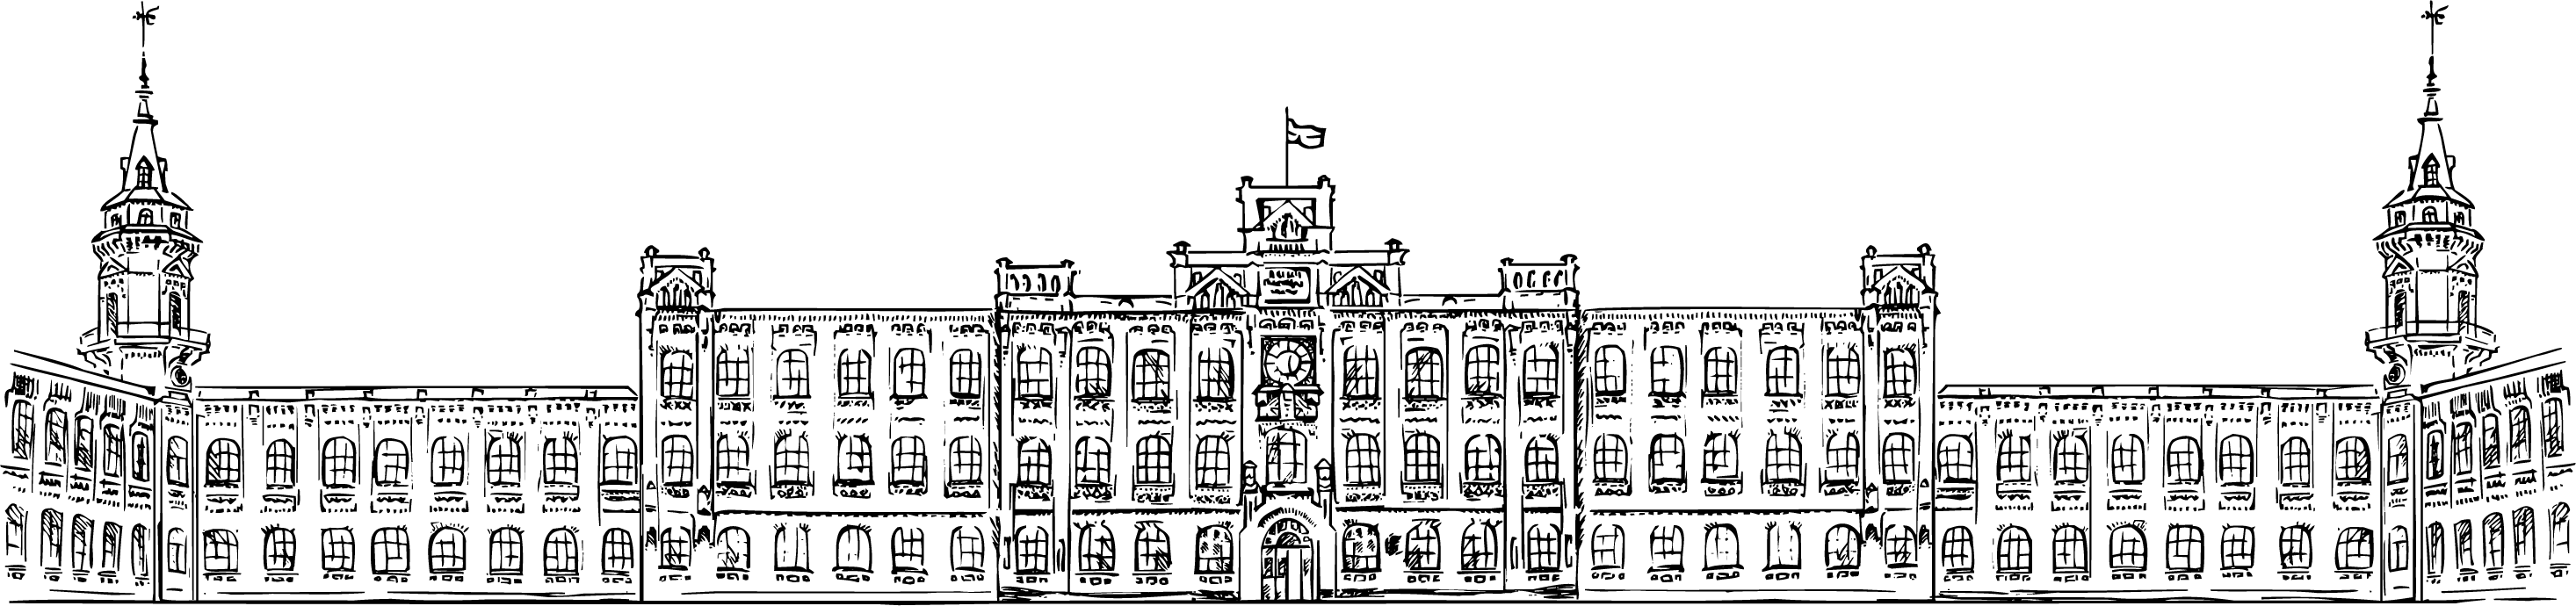
\includegraphics[width=0.7\textwidth]{../../../../../../templates/letterhead.png}\end{center}
  \begin{center}\large
    Національний технічний університет України\\
    «Київський політехнічний інститут імені Ігоря Сікорського»\\[1em]
    Факультет інформатики та обчислювальної техніки\\
    Кафедра обчислювальної техніки
  \end{center}
  \vfill
  \begin{center}
    \textbf{\LARGE Технології Computer Vision}\\[2em]
    \textbf{\Large Лабораторна робота №3}\\[0.7em]
    \parbox{0.9\textwidth}{\centering «Фільтрація та покращення якості цифрових зображень»}
  \end{center}
  \vfill
  \begin{flushright}\begin{minipage}{0.48\textwidth}
    Виконав: студент 3 курсу ФІОТ,\\
    групи \studentGroup\\
    \textit{\studentName}\\
    Залікова книжка № \recordBook\\[1em]
    Перевірив: \textit{\teacherName}
  \end{minipage}\end{flushright}
  \vfill
  \begin{center}Київ --- \reportYear\end{center}
\end{titlepage}

\pagenumbering{arabic}
\section{Тема та мета роботи}
\noindent\textbf{Тема:} фільтрація та покращення якості цифрових зображень.

\medskip
\noindent\textbf{Мета:} дослідити практичне застосування фільтрів, методів покращення якості та бінаризації для виділення будівель на двох супутникових знімках однієї території КПІ.

\section{Завдання роботи}
У роботі явно виконано завдання групи 3 методичних рекомендацій:
\begin{enumerate}[leftmargin=*,itemsep=0.2em]
  \item використати два знімки однієї території КПІ: Landsat/ArcGIS та Bing Maps;
  \item виконати grayscale-перетворення, GaussianBlur і покращення контрасту CLAHE;
  \item дослідити Otsu, адаптивну бінаризацію, Canny та кольорову маску;
  \item застосувати морфологічні операції для очищення масок;
  \item знайти контури, відфільтрувати їх за площею, співвідношенням сторін, extent, solidity та rectangularity;
  \item порівняти кількість отриманих кандидатів на двох знімках і вибрати відтворювану комбінацію операцій;
  \item зберегти маски, розмічені зображення та повний програмний лістинг.
\end{enumerate}

\section{Математична модель}
Растрове зображення подано як масив \(I\in\{0,\ldots,255\}^{H\times W\times3}\). Перехід до відтінків сірого виконується формулою
\begin{equation}
G(x,y)=0.299R(x,y)+0.587G(x,y)+0.114B(x,y).
\end{equation}
Коефіцієнти враховують різну чутливість людського зору до каналів: зелений канал має найбільшу вагу.

Гаусове розмиття є згорткою з ядром
\begin{equation}
K_\sigma(x,y)=\frac{1}{2\pi\sigma^2}\exp\left(-\frac{x^2+y^2}{2\sigma^2}\right).
\end{equation}
Воно зменшує дрібний шум перед виділенням меж.

Метод Otsu вибирає поріг \(T\), який максимізує міжкласову дисперсію. Після цього формується маска
\begin{equation}
B(x,y)=\begin{cases}255,&G(x,y)>T,\\0,&G(x,y)\leq T.\end{cases}
\end{equation}

Для контуру \(C_i\) обчислюються площа \(A_i\), bounding box \(w_i\times h_i\), extent та solidity:
\begin{equation}
\operatorname{extent}_i=\frac{A_i}{w_i h_i},\qquad
\operatorname{solidity}_i=\frac{A_i}{A(\operatorname{convexHull}(C_i))}.
\end{equation}
Контур приймається, якщо
\begin{equation}
A_{\min}\leq A_i\leq A_{\max},\quad r_{\min}\leq\frac{w_i}{h_i}\leq r_{\max},\quad
\operatorname{extent}_i\geq e_{\min},\quad\operatorname{solidity}_i\geq s_{\min}.
\end{equation}

\section{Архітектура програмного рішення}
\begin{figure}[H]\centering
\begin{tikzpicture}[node distance=0.45cm and 0.75cm,
  block/.style={draw,rounded corners,align=center,minimum width=3.3cm,minimum height=0.75cm,fill=blue!7},
  arrow/.style={-{Latex[length=2mm]},thick}]
  \node[block] (in) {Два знімки\\однієї території};
  \node[block,right=of in] (prep) {Grayscale, CLAHE,\\GaussianBlur};
  \node[block,right=of prep] (mask) {Otsu, adaptive,\\Canny, color mask};
  \node[block,below=of mask] (morph) {Opening/Closing\\та очищення маски};
  \node[block,left=of morph] (cont) {findContours\\та геометричні ознаки};
  \node[block,left=of cont] (out) {Розмітка, підрахунок\\і порівняння};
  \draw[arrow] (in)--(prep)--(mask)--(morph)--(cont)--(out);
\end{tikzpicture}
\caption{Архітектура програмного рішення}
\end{figure}

Для чесного порівняння обидва знімки проходять через однакову послідовність операцій. Відрізняються лише розмір, контраст і просторова деталізація самих вхідних даних.

\section{Структура проєкту}
\begin{verbatim}
lab3/
|-- src/main.py
|-- src/landsat.png
|-- src/bing.png
|-- results/landsat/
|-- results/bing/
|-- results/registered/
|-- results/summary.csv
|-- requirements.txt
`-- docs/main.tex
\end{verbatim}

\section{Результати роботи}
На рисунках 2--5 наведено вхідні знімки та проміжні результати обробки. Landsat/ArcGIS має більшу роздільність, тому окремі дахи частіше утворюють самостійні області. Bing має меншу роздільність, через що дрібні об'єкти сильніше зливаються з деревами та фоном.

\begin{figure}[H]\centering
  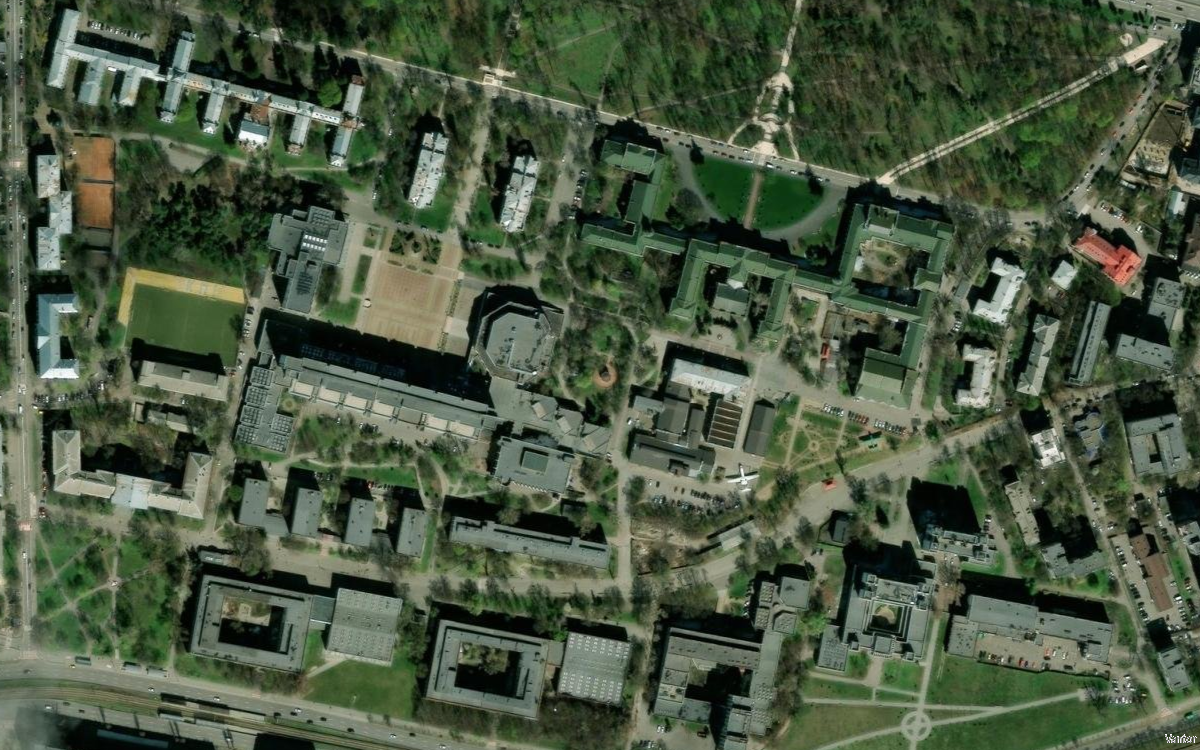
\includegraphics[width=0.96\textwidth]{../src/landsat.png}
  \caption{Вхідний знімок території КПІ з Landsat/ArcGIS}
\end{figure}
\begin{figure}[H]\centering
  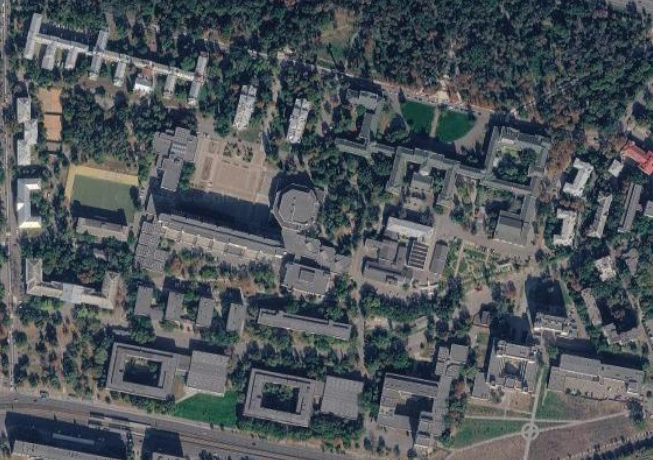
\includegraphics[width=0.80\textwidth]{../src/bing.png}
  \caption{Вхідний знімок тієї самої території з Bing Maps}
\end{figure}
\begin{figure}[H]\centering
  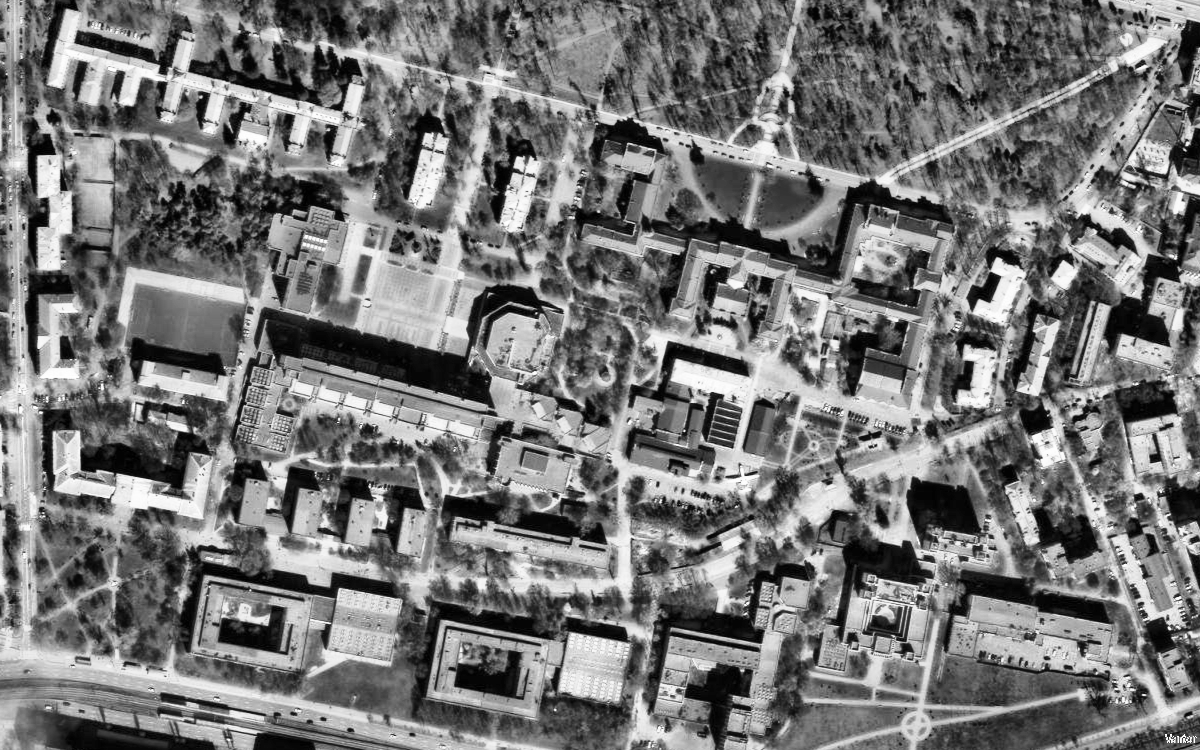
\includegraphics[width=0.96\textwidth]{../results/landsat/enhanced.png}
  \caption{Покращене grayscale-зображення Landsat/ArcGIS}
\end{figure}
\begin{figure}[H]\centering
  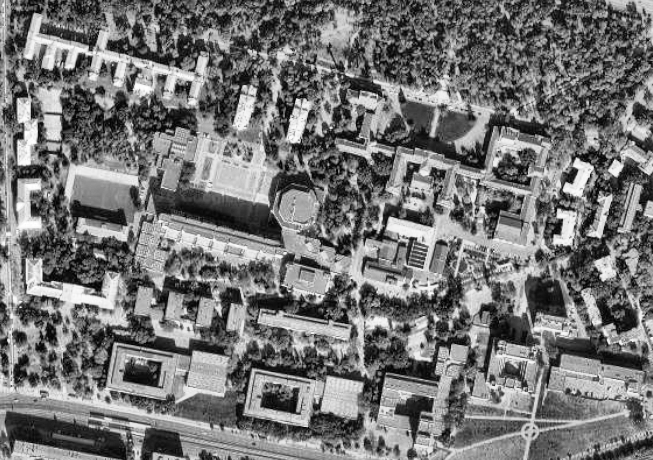
\includegraphics[width=0.80\textwidth]{../results/bing/enhanced.png}
  \caption{Покращене grayscale-зображення Bing Maps}
\end{figure}

\subsection{Проміжні маски та результати фільтрації}
Нижче наведено всі результати основних етапів, збережені програмою для двох знімків. Ліворуч у кожній парі розташовано результат для Landsat/ArcGIS, праворуч — для Bing Maps.

\methodpair{Grayscale-зображення}{../results/landsat/grayscale.png}{../results/bing/grayscale.png}
\methodpair{Маска адаптивної бінаризації}{../results/landsat/mask_adaptive.png}{../results/bing/mask_adaptive.png}
\methodpair{Результат адаптивної бінаризації}{../results/landsat/detected_adaptive.png}{../results/bing/detected_adaptive.png}
\methodpair{Кольорова маска}{../results/landsat/mask_color.png}{../results/bing/mask_color.png}
\methodpair{Результат кольорової маски}{../results/landsat/detected_color.png}{../results/bing/detected_color.png}
\methodpair{Маска Canny}{../results/landsat/mask_edges.png}{../results/bing/mask_edges.png}
\methodpair{Результат Canny}{../results/landsat/detected_edges.png}{../results/bing/detected_edges.png}
\methodpair{Маска Otsu}{../results/landsat/mask_otsu.png}{../results/bing/mask_otsu.png}
\methodpair{Результат Otsu}{../results/landsat/detected_otsu.png}{../results/bing/detected_otsu.png}
\methodpair{Комбінована маска Otsu + color}{../results/landsat/mask_otsu_color.png}{../results/bing/mask_otsu_color.png}
\methodpair{Результат Otsu + color}{../results/landsat/detected_otsu_color.png}{../results/bing/detected_otsu_color.png}
\methodpair{Комбінована маска adaptive + color}{../results/landsat/mask_adaptive_color.png}{../results/bing/mask_adaptive_color.png}
\methodpair{Результат adaptive + color}{../results/landsat/detected_adaptive_color.png}{../results/bing/detected_adaptive_color.png}
\methodpair{Маска consensus}{../results/landsat/mask_gray_consensus.png}{../results/bing/mask_gray_consensus.png}
\methodpair{Результат consensus}{../results/landsat/detected_gray_consensus.png}{../results/bing/detected_gray_consensus.png}
\methodpair{Основна комбінована маска}{../results/landsat/mask_final.png}{../results/bing/mask_final.png}
\methodpair{Основний комбінований результат}{../results/landsat/detected_final.png}{../results/bing/detected_final.png}

Для порівняння pipeline використано такі результати:
\begin{table}[H]\centering
\caption{Кількість кандидатів після геометричної фільтрації}
\begin{tabular}{lrr}
\toprule
Метод & Landsat/ArcGIS & Bing Maps\\
\midrule
Otsu & 22 & 27\\
Adaptive threshold & 10 & 32\\
Canny/edges & 53 & 4\\
Color mask & 56 & 21\\
Otsu + color & 51 & 27\\
Adaptive + color & 55 & 37\\
Основна комбінована маска & 40 & 16\\
Стабільний consensus після ORB/RANSAC & 35 & ---\\
\bottomrule
\end{tabular}
\end{table}

Метод Otsu та інші незалежні маски дають різну кількість кандидатів через відмінності масштабу й освітлення. Фінальний експеримент використовує стабільний consensus: знімки спочатку вирівнюються за ORB/RANSAC, а потім залишаються тільки області, які підтримуються обома джерелами. Для нового якіснішого Landsat-знімка отримано 35 геометричних кандидатів. Візуальний аудит показує, що частина з них все ще може бути фрагментом даху, дороги або іншого об'єкта, тому це не слід трактувати як гарантовану кількість будівель.

\begin{figure}[H]\centering
  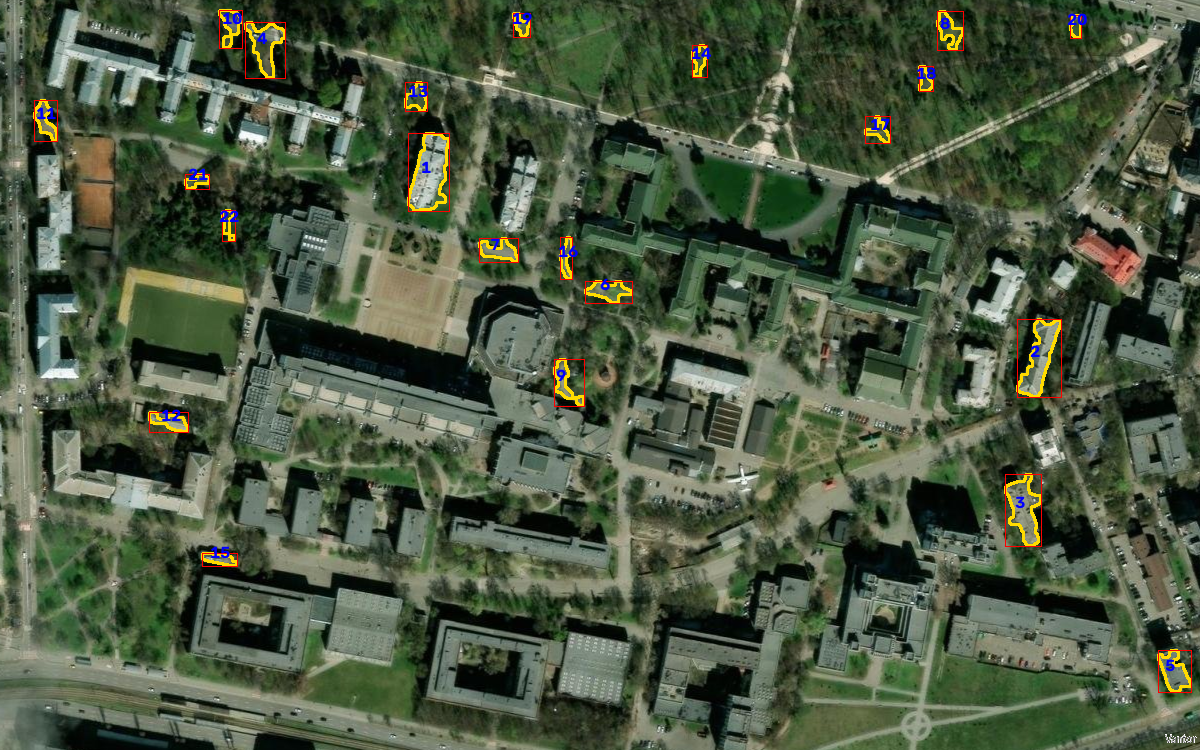
\includegraphics[width=0.96\textwidth]{../results/landsat/detected_otsu.png}
  \caption{Результат Otsu та геометричної фільтрації для Landsat/ArcGIS}
\end{figure}
\begin{figure}[H]\centering
  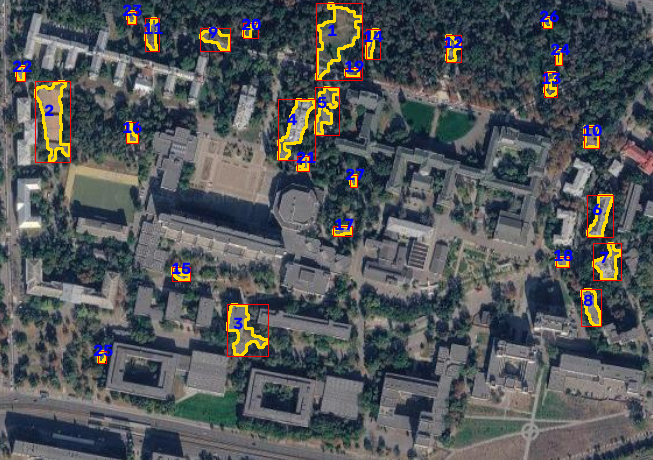
\includegraphics[width=0.80\textwidth]{../results/bing/detected_otsu.png}
  \caption{Результат Otsu та геометричної фільтрації для Bing Maps}
\end{figure}
\begin{figure}[H]\centering
  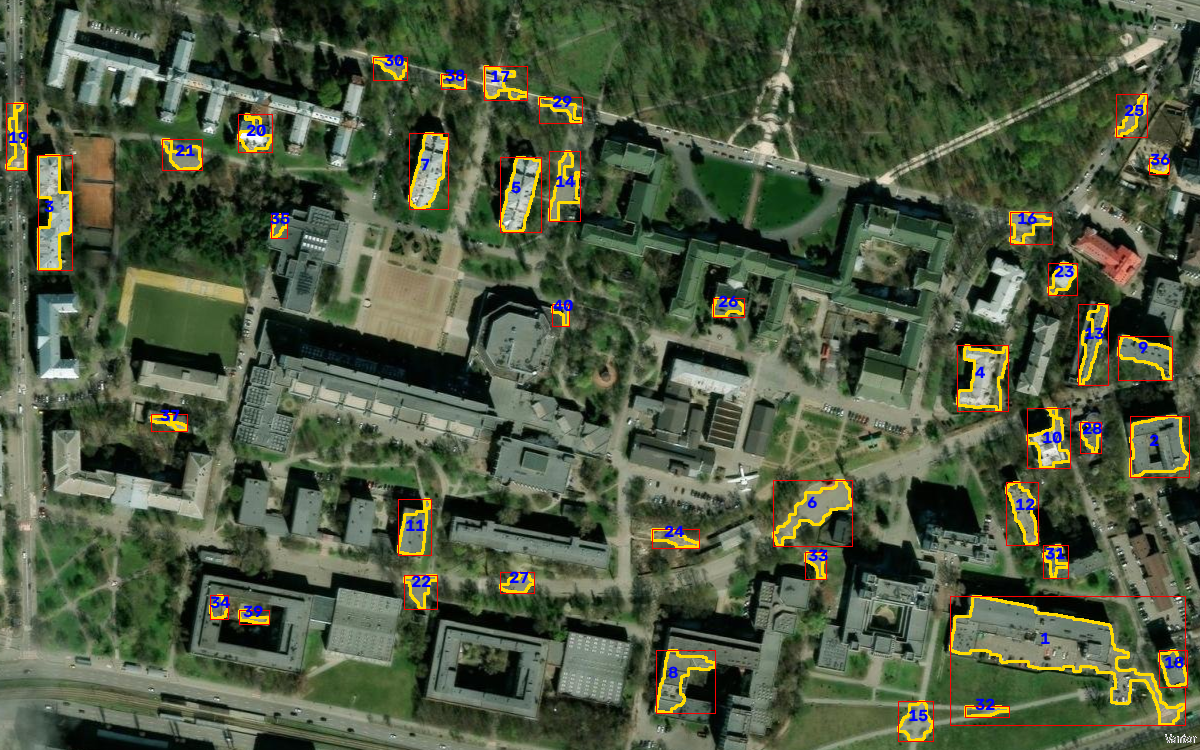
\includegraphics[width=0.96\textwidth]{../results/landsat/detected_final.png}
  \caption{Результат комбінованої маски для Landsat/ArcGIS}
\end{figure}
\begin{figure}[H]\centering
  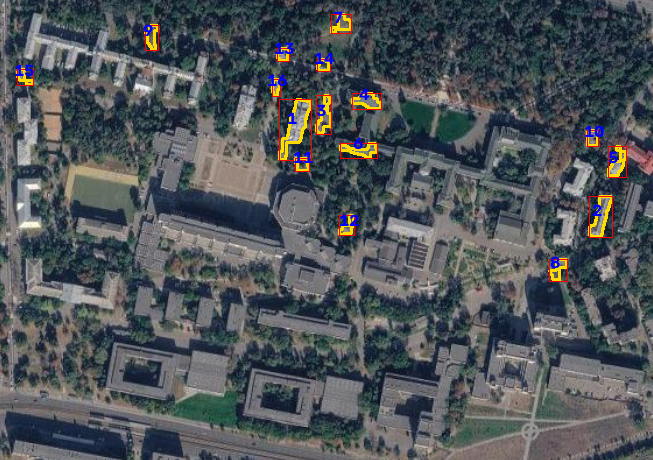
\includegraphics[width=0.80\textwidth]{../results/bing/detected_final.png}
  \caption{Результат комбінованої маски для Bing Maps}
\end{figure}
\begin{figure}[H]\centering
  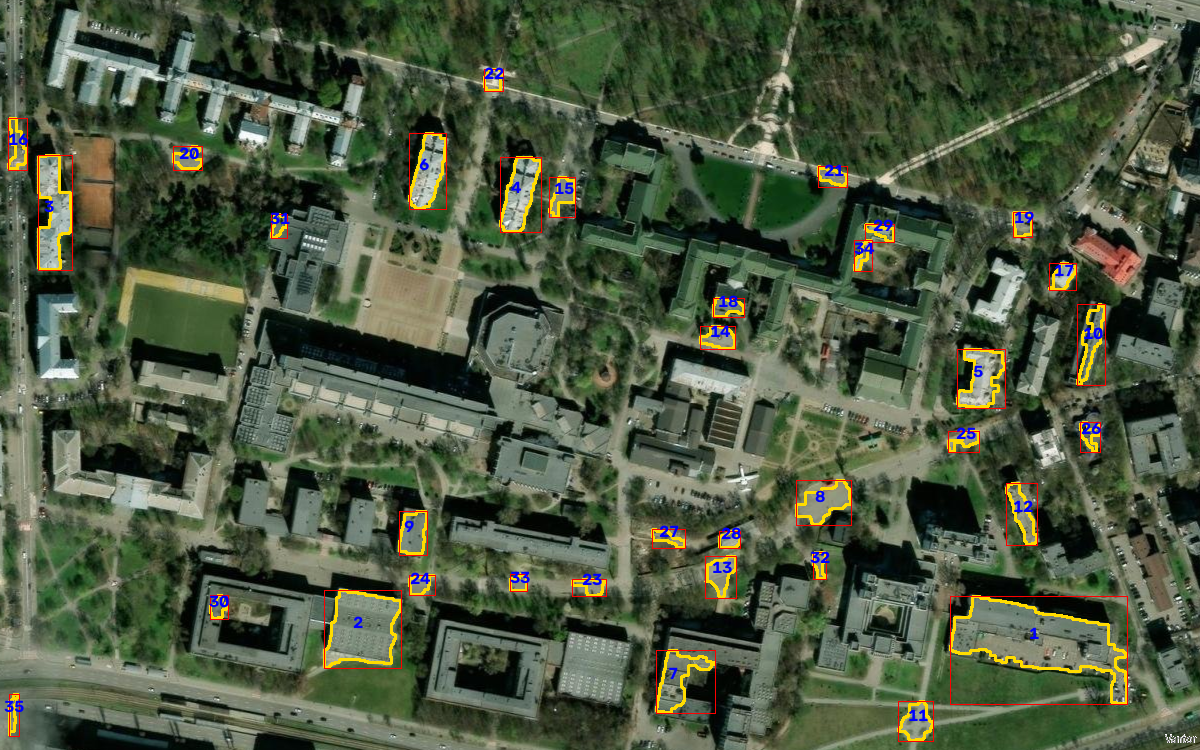
\includegraphics[width=0.96\textwidth]{../results/registered/stable_result.png}
  \caption{Фінальний стабільний результат після ORB/RANSAC та геометричної фільтрації}
\end{figure}

Для контролю узгодженості стабільного результату з Bing-baseline обчислено відносну різницю:
\begin{equation}
\delta=\frac{|N_{stable}-N_{Bing,Otsu}|}{N_{Bing,Otsu}}\cdot100\%=\frac{|35-27|}{27}\cdot100\%\approx29.6\%.
\end{equation}
Отже, новий Landsat-знімок покращив деталізацію, але різниця між джерелами залишається суттєвою. Це підтверджує, що класичний pipeline придатний для дослідження фільтрації та формування кандидатів, але не забезпечує точний семантичний підрахунок без ручної розмітки.


\section{Висновки}
У роботі реалізовано повний pipeline фільтрації: grayscale, CLAHE, GaussianBlur, бінаризацію, морфологічну обробку, ORB/RANSAC-вирівнювання, пошук контурів та геометричну фільтрацію. Новий PNG-знімок Landsat має кращу якість, але частина контурів усе ще не є гарантовано будівлями.

Отримані 35 і 27 — це кількість геометричних кандидатів на різних етапах, а не підтверджений кадастровий підрахунок. Для точного результату потрібні ручна розмітка або спеціалізована модель сегментації будівель.

\section{Лістинг програми}
\inputminted{python}{../src/main.py}

\end{document}
